\subsection{Wire with a constant curvature -- ring shaped wire}\label{sec:rings}

Here, we consider a flat anisotropic FM nanowire with a fixed cross-section of area $S$ and constant curvature -- ring shaped wire, see Fig.~\ref{fig:Geometries_n_curvatures}(a). The ring geometry is a prototypical example of a highly-symmetrical curved system with constant curvature $\varkappa=\text{const}$. It was investigated intensively both experimentally~\cite{Klaui01,Klaui03a,Klaui05a} and theoretically~\cite{Kravchuk09,Kravchuk11,Sheka15}.% due to the potential applications in magnetic storage media. To control the recording element it is necessary to have at least two different equilibrium magnetization states and well defined switching mechanism between them. In the case of magnetic nanorings made from soft magnetic materials the main equilibrium state is a \textit{vortex state} in which the magnetic flux is closed in the element.

\subsubsection{Equilibrium states}\label{sec:rings_equilibrium}

For the case ring-shaped nanowire with constant curvature, the minimization of energy~\eqref{eq:energy_angular} results in the solution $\theta_0=\pi/2$ and the azimuthal angle $\phi$, which
satisfies the pendulum equation
\begin{equation}\label{eq:ring_phi}
\phi'' - \sin\phi\cos\phi = 0.
\end{equation}
This equation has a trivial solution in curvilinear reference of frame which correspond to the \textit{vortex} magnetization distribution with
\begin{equation}\label{eq:ring_vortex}
\theta_0^\text{vor}=\pi/2,\quad \cos\phi_0^\text{vor} = \mathcal{C}=\pm 1,
\end{equation}
which is well known for the magnetic nanorings. Parameter $\mathcal{C}=\pm1$ is a chirality of the magnetization distribution, i.e $\mathcal{C}=+1$ and $\mathcal{C}=-1$ correspond to the clockwise and counterclockwise magnetization distribution, respectively. This state is typical for relatively large rings (rings with small curvature) and describes flux-free magnetization distribution, see Fig.~\ref{fig:ring_states}(a).

%==================================================================\
\begin{figure}[t]
	\centering
	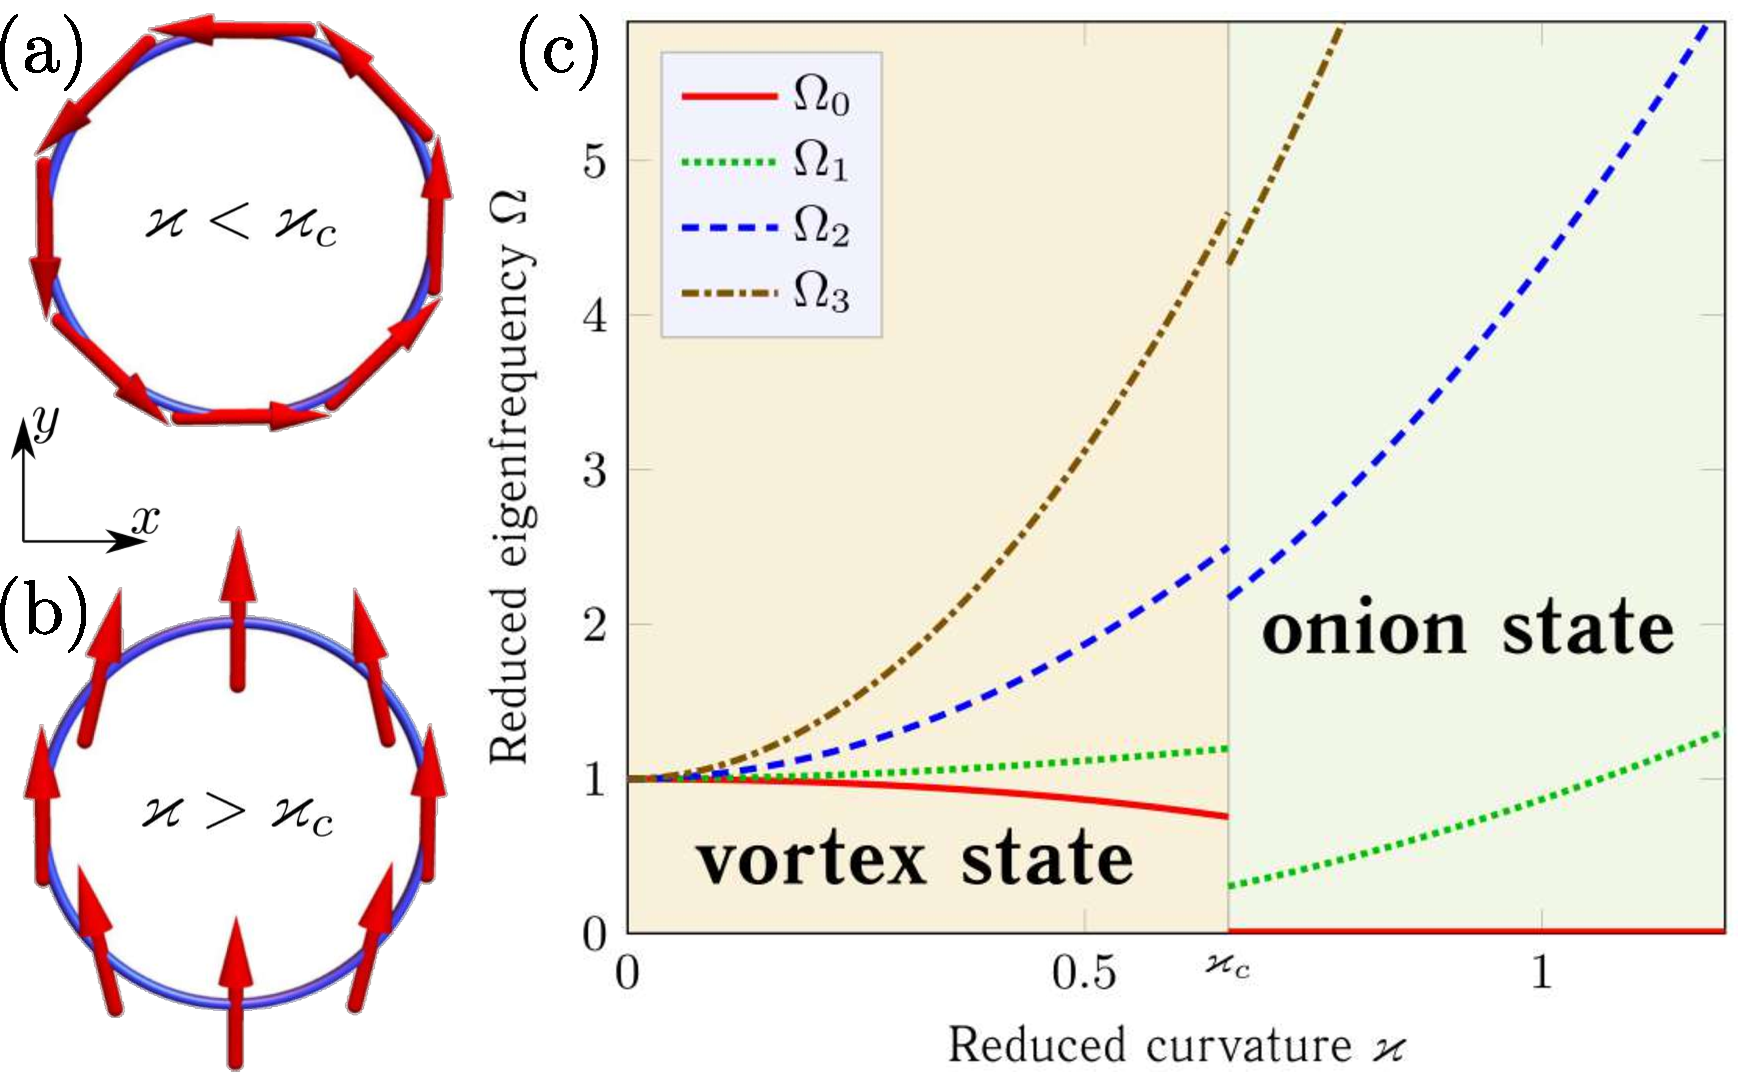
\includegraphics[width=0.8\textwidth]{fig_ring_states}
	\caption{\label{fig:ring_states}%
		\textbf{Nanoring wire:} Magnetization distribution of the ground state in a ring wire with different reduced curvatures: (a) vortex state for $\varkappa<\varkappa_c$ and (b) onion state for $\varkappa>\varkappa_c$. (c) The lowest eigenfrequencies of linear excitations in a ring nanowire depending on the curvature $\varkappa$. Adapted with permission from~\cite{Sheka15}.}
\end{figure}
%==================================================================/

Equation~\eqref{eq:ring_phi} also has an inhomogeneous solution in curvilinear reference of frame
\begin{equation}\label{eq:ring_onion}
\theta_0^\text{on}=\pi/2,\quad \phi_0^\text{on}(\xi)=\text{am}\left[\xi/k,k\right].
\end{equation}
where $\text{am}\left(x,y\right)$ is the Jacobi amplitude~\cite{NIST10} and the modulus $k$ is determined by the condition $2\varkappa k \mathrm{K}(k)=\pi$ with $\mathrm{K}(k)$ being the complete elliptic integral of the first kind~\cite{NIST10}. This state is characterized with a quasi-uniform magnetization distribution in Cartesian reference of frame, see Fig.~\ref{fig:ring_states}(b). This state is an arrangement of magnetic moments in which the ring is divided into two magnetic domains separated by two domain walls, with magnetization oriented tangentially in two different directions, clockwise and counterclockwise. This structure is usually referred to as an \textit{onion} state~\cite{Klaui03a}.  One should note that for the case of magnetoelastic rings, the onion state~\eqref{eq:ring_onion} results in deformation of the ring shape from circular to the elliptic-like geometry~\cite{Gaididei19}.

Both \textit{vortex} and \textit{onion} equilibrium states correspond to the planar magnetization distribution within the wire plane.

Nanorings with \textit{vortex} magnetization ground state can be prepared with smaller radii than nanodisks with the same magnetization structure~\cite{Kravchuk07}. The critical radius which separates the \textit{vortex} and \textit{onion} states defined, in general, by the relation $\varkappa_c \approx 0.657$~\cite{Sheka15}. For the permalloy nanoring we have  critical radius $R_{c}\approx 17$ nm, i.e. for rings with $R>R_c$ one obtains \textit{vortex} state, while for $R<R_c$ -- \textit{onion} state.

%As it was mentioned above, two domains in the \textit{onion} state are separated by two domain walls. Depending on the width of the ring one can obtain a transverse head-to-head~(tail-to-tail) DWs for narrow ribbons, or vortex head-to-head~(tail-to-tail) domain walls for wide rings, see Fig.~\ref{fig:ring_states}.

\subsubsection{Magnon spectrum in the ferromagnetic ring}\label{sec:ring_eigenmodes}

In the Sec.~\ref{sec:theory_1D} it is shown that nontrivial geometry results in appearance of the effective exchange-driven DMI and anisotropy. Therefore, one should expect the modification of magnon spectrum similar to the systems with an intrinsic DMI. To analyse the magnons in the curved system, we linearize the LLG equation~\eqref{eq:llg_angular} for zero damping $\alpha_\textsc{g}=0$ on the background of the vortex~\eqref{eq:ring_vortex} and onion~\eqref{eq:ring_onion} states with the substitution $\theta=\theta_0+\vartheta(\overline{t},\xi)$ and $\phi=\phi_0+\varphi(\overline{t},\xi)$. The linearizaed equations of motion reads as~\cite{Sheka15,Gaididei18a,Korniienko19b}
\begin{equation}\label{eq:ring_magnons}
-\vartheta''+V_1\vartheta = \dot{\varphi},\quad  -\varphi''+V_2\varphi = -\dot{\vartheta},
\end{equation}
where $V_1 = \cos^2\phi_0 - \left[\phi_0'+\varkappa(\xi)\right]^2$ and $V_2 = \cos2\phi_0$ are geometry-induced potentials.

For the simplest case of the ring-shaped wire with constant curvature $\varkappa=\text{const}$ and \textit{vortex} magnetization distribution one obtain $V_1=1-\varkappa^2$ and $V_2=1$. The set~\eqref{eq:ring_magnons} can be solved with plane waves ansatz $\vartheta=\sum_j \vartheta_j \cos(j\xi\varkappa-\Omega\overline{t}+\delta_j)$ and $\varphi=\sum_j \varphi_j \sin(j\xi\varkappa-\Omega\overline{t}+\delta_j)$ with $j$ being the azimuthal quantum number, $\delta_j$ is an arbitrary phase, and $\Omega$ is dimensionless frequency measured in units $\omega_0$. By substituting this ansatz in the set~\eqref{eq:ring_magnons} we can calculate the spectrum of magnon eigenstates as
\begin{equation}\label{eq:spec_rings}
\Omega^\text{vor}_j = \sqrt{\left(V_1+j^2\varkappa^2\right)\left(V_2+j^2\varkappa^2\right)}.
\end{equation}
The corresponding lower eigenfrequencies are plotted in the Fig.~~\ref{fig:ring_states}(c). For the limit case of the small curvature $\varkappa\ll1$~(quasi-straight wire), the magnon frequencies read
\begin{equation}\label{eq:spec_rings_small}
\Omega^\text{vor}_j = 1- \frac{\varkappa^2}{2}+j^2\varkappa^2+\mathcal{O}(\varkappa^4).
\end{equation}
Thus the curvature decreases the gap as compared to the case of the straight wire~($\varkappa=0$) with dispersion $\Omega^\text{str} = 1 + \mathfrak{K}^2$, where $\mathfrak{K}=j\varkappa$ is the corresponding normalized wave vector.

For the case of the \textit{onion} magnetization distribution \eqref{eq:ring_onion} the corresponding lower eigenfrequencies can be estimated as~\cite{Sheka15}
\begin{equation}\label{eq:spec_rings_onion}
	\Omega^\text{on}_j = \sqrt{\left(\mathcal{V}_1+j^2\varkappa^2\right)\left(\mathcal{V}_2+j^2\varkappa^2\right)},
\end{equation}
where $\mathcal{V}_1 = 1/k^2 + \varkappa^2 - 4\varkappa\mathrm{E}(k) /\left(k\pi\right)$ and  $\mathcal{V}_2 = 2/k^2 - 1 - 4\varkappa\mathrm{E}(k) /\left(k\pi\right)$ are first terms in the Fourier expansions of potential $V_1$ and $V_2$, respectively. Here, $\mathrm{E}(k)$ is the complete elliptic integral of the second kind~\cite{NIST10}. The corresponding lower eigenfrequencies are plotted in the Fig.~\ref{fig:ring_states}(c). Equation~\eqref{eq:spec_rings_onion} does not take into account the modes coupling, which can lead in the mixing of different partial waves.

The limit case $\Omega^\text{on}_0 = 0$ corresponds to the zero (Goldstone) mode, which is realized due to the arbitrary direction of the onion axis. Here, Goldstone mode contains an infinite number of partial waves; hence the coupling between different partial waves for this mode is crucial~\cite{Sheka15}.